\chapter{Software Process, Software Design, Implementation and Testing}

\section{Software Process}

I followed an Agile approach in my project because the requirements for my project evolved as I progressed, as I researched more and learnt more about the area I had more ideas about what I wanted to include and having an Agile approach allowed me to incorporate these ideas. 

For the first week I followed the Kanban process and used the online tool Glo Boards\cite{glo_board}, I however quickly realised that Kanban was not the right process to use because Kanban is generally about improving an already established process and as I was just starting I didn't have a process to improve so it didn't make a huge amount of sense to follow. 

I soon switched to using Scrum, this made a lot more sense because the project generally follows the design of a Scrum project already. I had sprints that lasted a week because each week I would have a meeting and you could consider this meeting to be a sort of extended stand-up, I discussed and demoed what I had worked on and we discussed what I could get done by next week. The product owner was me because I was ultimately in charge of the direction of the project and what new areas it would cover, my supervisor obviously had a guiding hand in what would be developed each week and what good progress would be.

When I switched to Scrum I realised that Glo Boards weren't really working for me so I switched to using Jira\cite{jira_site}. I made heavy use of epics to group my work and epics didn't work the way I wanted them to in Glo Boards. Jira was a tool that I used during my Industrial Year and I felt that it was very useful in planning and keeping track of work. I organised my work into epics and through the use of the backlog tool and the sprint management tool it was easy to see how well I was progressing and what still needed to be done. Figure \ref{fig:jira_epics} shows how Jira lays out epics in its road map view.

\begin{figure}
    \centering
    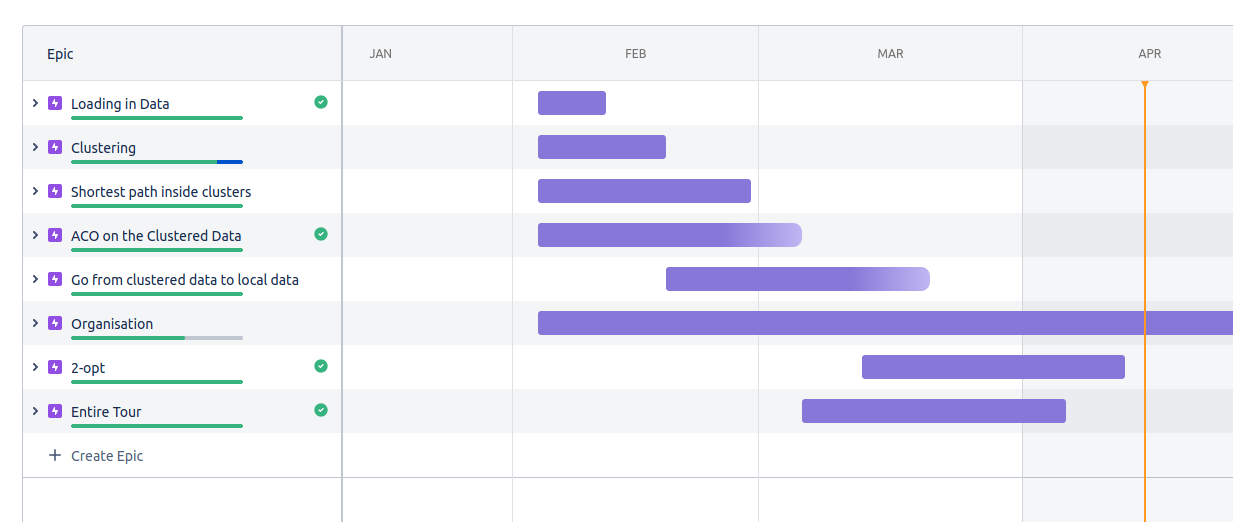
\includegraphics[width=\textwidth]{Project Report/LaTeX Template/figures/jira_epics.png}
    \caption{Figure showing how the work was divided into epics in Jira, each epic had a number of tasks associated to it, when all of these tasks where completed the epic could be then be marked as done. This image was taken late into the project when most of the work had been done.}
    \label{fig:jira_epics}
\end{figure}

In Jira I assigned each task a story point estimate, this was a number between 0 and 3 that represented how much work that task would be to accomplish, 0 being very little work and 3 being a substantial amount of work normally several days. In Jira I could then generate a burndown report which could visualise how many story points I process through in a sprint and whether I was assigning myself a good amount of work each sprint. figure \ref{fig:jira_burndown} shows how this burndown chart looks in Jira.

\begin{figure}
    \centering
    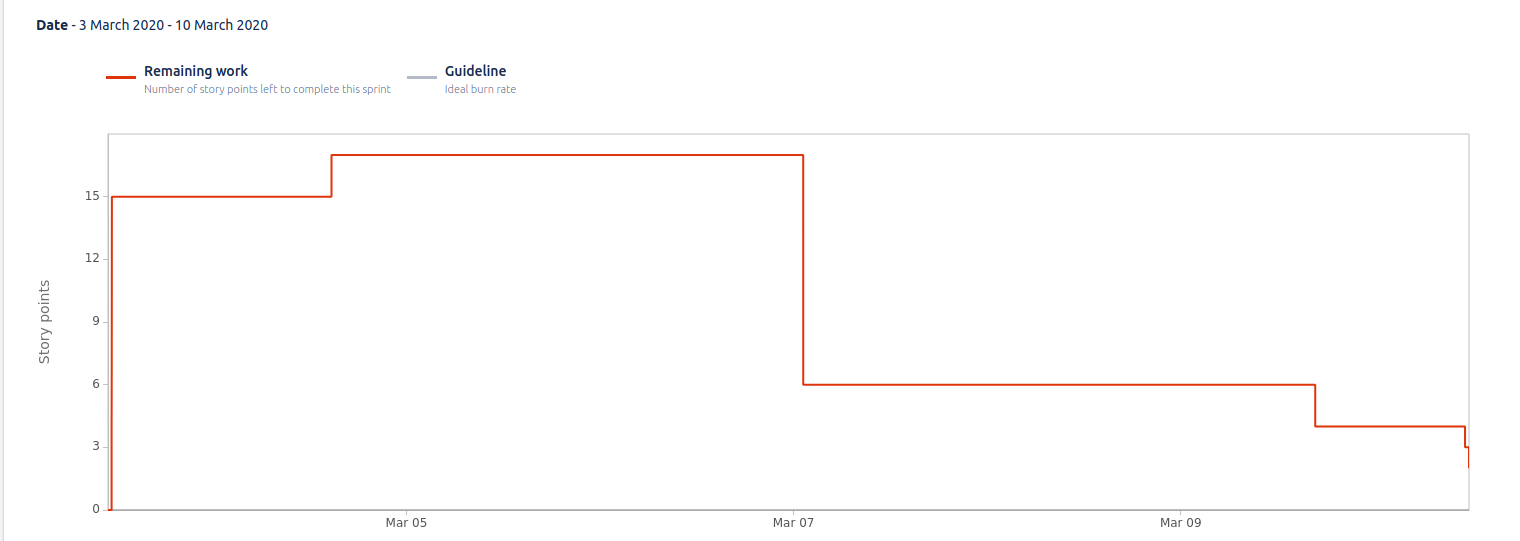
\includegraphics[width=\textwidth]{Project Report/LaTeX Template/figures/jira_sprint_burndown.png}
    \caption{Figure showing Sprint burndown chart in Jira, this allows you to visualise how much work you normally accomplish on a given sprint and allow you to better plan your future sprints by allocating an appropriate amount of work. You can see in this sprint I started with 15 story points but after re-estimating a task that was raised to 17, I then managed to do most of that work and ended the sprint with 1 task left that had a story point estimate of 2.}
    \label{fig:jira_burndown}
\end{figure}

This could be one chapter or a few chapters. It should define and discuss the software that is developed to support the research that is being conducted. For example, if your research involves running experiments, what software are you creating to support that work? What functionality is required? What design will be used? What implementation issues are there and what testing is used? 

Even though a research project is investigating specific research questions, it is still necessary for you to discuss the software that you develop. Research has a habit of generating bits of software that can exist for several years and need future modification. Therefore you need to be able to discuss the technical issues as well as the research approach. 

\section{Design}
You should concentrate on the more important aspects of the design. It is essential that an overview is presented before going into detail. As well as describing the design adopted it must also explain what other designs were considered and why they were rejected.

The design should describe what you expected to do, and might also explain areas that you had to revise after some investigation.

Typically, for an object-oriented design, the discussion will focus on the choice of objects and classes and the allocation of methods to classes. The use made of reusable components should be described and their source referenced. Particularly important decisions concerning data structures usually affect the architecture of a system and so should be described here.

How much material you include on detailed design and implementation will depend very much on the nature of the project. It should not be padded out. Think about the significant aspects of your system. For example, describe the design of the user interface if it is a critical aspect of your system, or provide detail about methods and data structures that are not trivial. Do not spend time on long lists of trivial items and repetitive descriptions. If in doubt about what is appropriate, speak to your supervisor.
 
You should also identify any support tools that you used. You should discuss your choice of implementation tools - programming language, compilers, database management system, program development environment, etc.

Some example sub-sections may be as follows, but the specific sections are for you to define. 

\subsection{Overall Architecture}

\subsection{Some detailed design}

\subsubsection{Even more detail}

\subsection{User Interface}

\subsection{Other relevant sections}

\section{Implementation}

This section should discuss issues you encountered as you tried to implement your experiments. What were the results of running the experiments? What conclusions can you draw from these results? 

During the work, you might have found that elements of your experiments were unnecessary or overly complex; perhaps third-party libraries were available that simplified some of the functions that you intended to implement. If things were easier in some areas, then how did you adapt your project to take account of your findings?

It is more likely that things were more complex than you first thought. In particular, were there any problems or difficulties that you found during implementation that you had to address? Did such problems simply delay you or were they more significant? 

If you had multiple experiments to run, it may be sensible to discuss each experiment in separate sections. 

\section{Testing}
Detailed descriptions of every test case are definitely not what is required in this section; the place for detailed lists of tests cases is in an appendix. In this section, it is more important to show that you adopted a sensible strategy that was, in principle, capable of testing the system adequately even if you did not have the time to test the system fully. 

Provide information in the body of your report and the appendix to explain the testing that has been performed. How does this testing address the requirements and design for the project?

How comprehensive is the testing within the constraints of the project?  Are you testing the normal working behaviour? Are you testing the exceptional behaviour, e.g. error conditions? Are you testing security issues if they are relevant for your project?

Have you tested your system on ``real users''? For example, if your system is supposed to solve a problem for a business, then it would be appropriate to present your approach to involve the users in the testing process and to record the results that you obtained. Depending on the level of detail, it is likely that you would put any detailed results in an appendix. 

Whilst testing with ``real users'' can be useful, don't see it as a way to shortcut detailed testing of your own. Think about issues discussed in the lectures about until testing, integration testing, etc. User testing without sensible testing of your own is not a useful activity.

The following sections indicate some areas you might include. Other sections may be more appropriate to your project. 

\subsection{Overall Approach to Testing}

\subsection{Automated Testing}

\subsubsection{Unit Tests}

\subsubsection{User Interface Testing}

\subsubsection{Stress Testing}

\subsubsection{Other types of testing}

\subsection{Integration Testing}

\subsection{User Testing}
